\documentclass[tikz,border=10pt]{standalone}
\usepackage{tikz}
\usetikzlibrary{intersections, calc}

\begin{document}

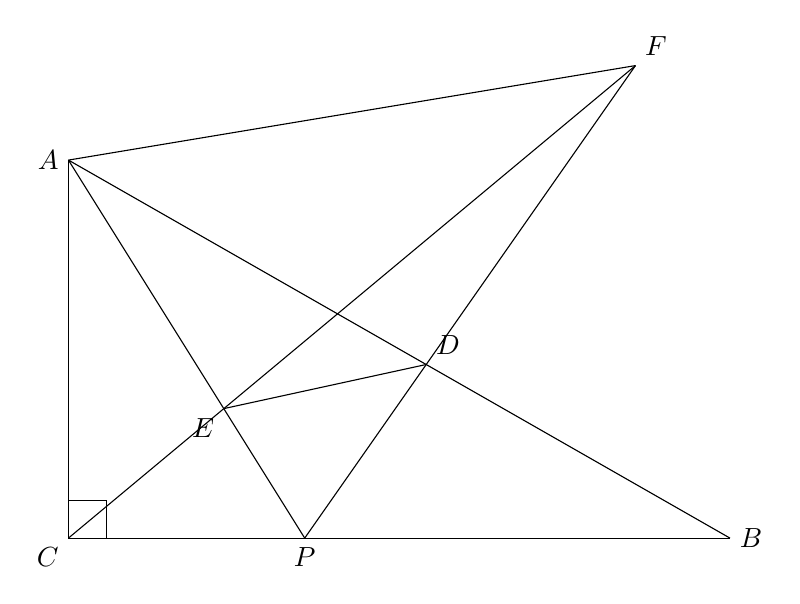
\begin{tikzpicture}[scale=1.2]
    % Define coordinates
    \coordinate (C) at (0,0);
    \coordinate (A) at (0,4);
    \coordinate (B) at (7,0);
    \coordinate (P) at (2.5,0);
    \coordinate (F) at (6,5);

    % Calculate intersections
    % Line AP
    % Line CF
    \coordinate (E) at (intersection of A--P and C--F);
    
    % Line AB
    % Line PF
    \coordinate (D) at (intersection of A--B and P--F);

    % Draw lines
    \draw (A) -- (C);
    \draw (C) -- (B);
    \draw (A) -- (B);
    \draw (A) -- (P);
    \draw (C) -- (F); % Passes through E
    \draw (P) -- (F); % Passes through D
    \draw (A) -- (F);
    \draw (E) -- (D);

    % Right angle mark at C
    \draw (0,0.4) -- (0.4,0.4) -- (0.4,0);

    % Labels
    \node[left] at (A) {$A$};
    \node[right] at (B) {$B$};
    \node[below left] at (C) {$C$};
    \node[below] at (P) {$P$};
    \node[above right] at (F) {$F$};
    \node[below left] at (E) {$E$};
    \node[above right] at (D) {$D$};

\end{tikzpicture}

\end{document}
